
\chapter{Systems - Beechcraft Duchess BE-76}

\emph{Models: N6001Y ME-119; N3733G ME-364}

\section{Engines}

The Duchess has two Lycoming 4 cylinder-engines – an O360 on the left, and an LO-360 (the ``L'' is for ``left'' turning) on the right. Both engines produce 180 horsepower at 2700 RPM and are air-cooled, direct drive,
horizontally opposed, reciprocating, normally aspirated engines. Oil capacity is 8 quarts maximum.

\section{Propellers}

\subsection{Propeller System Basics}

The Duchess has two 76-inch diameter, constant speed, full-feathering Hartzell propellers. The propellers are
counter-rotating: the left propeller turns clockwise and right propeller turns counterclockwise. Unlike most light
twins which have conventional propellers where both turn clockwise, there is no critical engine with counter-
rotating propellers. See the definition of critical engine in Section 1.

The propeller controls on the control console allow the pilot to select the governor's RPM range. Propeller governors
regulate oil pressure to control RPM by varying the blade angle (pitch) of the propeller to make it more efficient.
Oil pressure and aerodynamic twisting send the propeller out of feather to high RPM settings (low pitch=small blade
angle, taking small ``bites'' of air). Nitrogen pressure and a large spring, aided by counterweights, send the propeller
to low RPM (high pitch=high blade angle).

The oil pressure and nitrogen/spring pressure constantly oppose each other. When the propeller control is moved to
the feather position, the opposing oil pressure is released and the spring, air pressure and counterweights cause the
propeller to ``feather'' - a pitch of approximately 80\degree; this is a minimum drag condition. The propellers can be
unfeathered with the aid of unfeathering accumulators. When the propeller control is moved forward, stored oil
pressure is released which forces the propeller into a lower pitch. If this is done above 100 knots, the propeller
should windmill, allowing the engine to be re-started without the aid of the starter.

A feathering lock, operated by centrifugal force, prevents feathering during engine shut down by making it
impossible to feather any time the engine speed falls below 950 RPM. For this reason, when the pilot wishes to
feather a propeller, he must be sure to move the propeller control into the FEATHER position before the engine
speed drops below 950 RPM. This will not happen while airborne since the propeller will windmill faster than 950
RPM with normal propeller control settings. \emph{(see schematic)}

\subsection{Propeller Governor Operation}

The propeller governor is mounted on the accessory case on the rear of the engine. It contains a speeder spring,
which is directly controlled by the propeller lever in the cockpit, and flyweights which spin at engine RPM (see
propeller system diagram). When the pilot sets an RPM value with the propeller control, the engine attempts to
maintain that RPM setting by pitching the blades as required by the existing airspeed and power setting.

The propeller governor operates by regulating the flow of high-pressure oil into and out of the propeller hub.
Increasing oil pressure into the hub pitches the propeller blades flatter (higher RPM) and allowing oil to flow out of
the propeller hub allows the propeller to achieve a higher pitch (lower RPM or feather). The flow of oil is controlled
by a pilot valve in the governor which blocks the flow of oil to and from the propeller hub under normal conditions.

When the propeller RPM starts to increase (because of a momentary dive, for example) the flyweights are slung
away from the rotating shaft because of centrifugal force. This raises the shaft, which allows oil to flow from the
propeller hub to the oil sump, moving the blades to higher pitch and reestablishing the set RPM value. When the
propeller RPM starts to decrease, the counterweights have less centrifugal force slinging them away from the shaft,
and the speeder spring forces them inward. This moves the pilot valve in the opposite direction, which allows the
flow of high-pressure oil into the propeller hub, moving the blades to a flatter position and increasing RPM to the set
value.

At lower power settings and airspeeds, the propellers may be fully flat and RPM will decrease below the set value.
At this point, moving the propeller control fully forward will have no effect on engine RPM, since the blades are
already at their flattest pitch. This is called the governing range and is why the throttles change RPM when at idle.

\section{Landing Gear}

The retractable tricycle landing gear uses shock absorbers on the main gear (approximately 2" extension) and an
oleo strut on the nose gear (approximately 4 1/4" extension) for shock absorption. The nose gear is steerable
through a spring-loaded linkage connected to the rudder pedals. A hydraulic dampener on the nose strut eliminates
shimmy. Toe brakes aid in steering the aircraft. The minimum wingtip turn radius is approximately 27' with the use
of differential power.

Retraction and extension of the gear is accomplished through the use of an electrically driven reversible hydraulic
pump and hydraulic system terminating in a hydraulic actuator assembly mounted in each wheel well. Retraction or
extension requires 6-8 seconds. The gear is held in the retracted position by 1250 to 1550 PSI of hydraulic pressure;
there are no locks to hold the gear in the retracted position. The landing gear may be hydraulically extended or
retracted, and may be lowered manually (below 100 knots) by turning a dump valve which releases pressure from
the retract side of the system allowing the gear to free fall to the down and locked position. If you lose hydraulic
pressure for some other reason, the gear will lower (free fall) to the down position and you will not be able to raise
it. If you lose electrical power the gear can be lowered manually but not raised. For any gear malfunction
ALWAYS refer to the checklist.

\emph{Memory aid: Gear is electrically driven, hydraulically actuated. Pressure holds the gear up. Lack of pressure causes gear to free fall,
allowing us to drop gear in an emergency.}

Three green lights, one for each landing gear, are illuminated whenever the landing gear is down and locked. The
red light illuminates any time the gear is in-transit, indicating that the hydraulic pump is active. All of the lights will
be extinguished when the gear is up. Pressing the face of each indicator light will verify that the lights are
functional. The intensity of the lamps can be controlled by turning the lens holder on each lamp (counterclockwise
is brighter, full clockwise will appear that the bulb is out). In addition, the 4 gear indicator lights are
interchangeable with each other to verify that you do not have a burned out bulb.

In the retract mode the electric pump/motor forces hydraulic fluid to the retract side of the system. A pressure
switch shuts off the motor (and extinguishes the red in-transit light) when the system pressure reaches approximately
1550 PSI. If pressure drops to approximately 1250 PSI the motor will again be activated, and the red in-transit light
will illuminate. An uplock check valve in the pump retains this pressure to hold the gear up. In addition, landing
gear retraction operation is protected by a time-delay relay, which will disengage electrical power to the pump/motor
after 30 seconds of continuous operation. If the landing gear in-transit light remains illuminated, it indicates
improper response of the landing gear. The relay can be reset by moving the gear switch to the down position.

\emph{Memory aid: Watch for gear in-transit light illuminating in flight, this could indicate a failing pump or a leak in the system.}

In the extend mode the electric motor forces hydraulic fluid to the extend side of the system. Main gear downlock is
accomplished by over-center travel of a spring-held side brace. Nose gear downlock is accomplished by over-center
travel of the drag link and a mechanically actuated downlock. After the gear are down and locked, system pressure
will bleed back to zero. Down limit switches, located on each gear, will allow the pump/motor to run until all three
gear are down and locked.

To prevent inadvertent retraction of the landing gear on the ground, a safety pressure switch is installed in the pitot
system to deactivate the hydraulic pump circuit when impact air pressure is below approximately 59 to 63 knots.

\emph{Note: We do touch-and-gos faster than 61 knots: IDENTIFY/VERIFY.}

%\emph{Memory aid: Do not retract the gear on the ground! What if the safety pressure switch is inoperative?}

If either or both throttles are retarded below an engine setting sufficient to sustain flight and the landing gear are not
fully extended, the landing gear warning horn will sound intermittently. An optional gear warning silence button
\emph{(not installed in either of the PCA Duchess aircraft as of this writing)}
allows the pilot to silence the alarm if one throttle is retarded. Additionally, when the flaps are extended beyond
about 16\degree, the warning horn will sound, regardless of throttle position, if the landing gear is not down and locked.
\emph{(see schematic)}

System Operation Notes. For example:
\begin{enumerate}
\item The pilot moves the propeller control forward, which applies pressure from the speeder spring.
\item Flyweights and speeder spring move the pilot valve.
\item Oil from the engine driven governor oil boost pump is pushed toward the pilot valve.
\item Oil moves past the pilot valve toward the propeller hub.
\item Oil fills the propeller hub in the direction of the low pitch stop.
\item The low pitch stop sets the high RPM limit.
\end{enumerate}

The reverse is true when pulling the propeller lever aft to the low RPM range.

\section{Brakes and Tires}

Single-disk, double-piston Cleveland hydraulic brakes are fitted to the main gear. Each rudder pedal is fitted with a
master cylinder, which pressurizes the two pistons on either of the brake assemblies, forcing the linings to press
against the disk. To set the parking brake, pull the control out and pump both toe pedals until solid resistance is felt.
Push the control in to release the brakes. The hydraulic brake fluid reservoir is accessible through the nose
compartment. Fluid level is checked with the attached dipstick. The hydraulic system for the brakes is independent
of the gear. The main gear has 6.00-6 tires, and the nose gear has 5.00-5 tires. Normal inflation is 38 PSI for all
tires.

\section{Flaps and Trim}

Electrically actuated wing flaps are controlled by a three-position switch: UP, OFF, and DOWN. A dial type
indicator has position markings for UP, 10, 20, and DN (max is 35\degree{}). Limit switches interrupt power to the motor
when the flaps reach the extremes of travel. Intermediate flap positions can be obtained by placing the switch in the
off position during extension or retraction. Additionally, there is a micro switch activated at the 16\degree{} position which
is connected to the gear and stall warning circuits.

The elevator and rudder have cable-operated flight-adjustable trim tabs. The aileron control system has a trimmer
which functions by applying tension on the aileron control cables. Each control incorporates a mechanical position
indicator. The elevator trim may be operated manually or electrically.

\emph{Memory aid: $V_{FE}$ 120 KIAS @ 10 \degree{} - 20 \degree{}, 110 KIAS @ 35 \degree.}

\section{Pressure (Pneumatic) System}

Pressure for the attitude indicator and directional gyro is supplied by two engine-driven dry pressure pumps,
interconnected to form a single system. This is different from many light planes, which use vacuum to draw air
through the gyro instruments. If either pump fails, check valves automatically close and the remaining pump
continues to pressurize the system. Two red buttons on the pressure gauge indicate if that pump has failed. The HSI
is operated by the electrical system and therefore is not affected by a failure in the vacuum system.
\emph{(see schematic)}

\section{Pitot-Static System}

The Pitot tube is located outboard on the left wing. Pitot heat is available. The pitot system incorporates a pressure
switch, which prevents inadvertent gear retraction under approximately 60 knots. Static air is taken from flush static
ports located on each side of the fuselage. The alternate static air source is selectable on the lower left sidewall.
This lever also functions as the static system drain.

\section{Stall Warning System}

A stall warning sensing vane is installed on the leading edge of each wing. With flap settings of 0-15\degree{} the vane on
the left wing activates the warning horn. With flap settings of 16\degree{} or more the vane on the right wing activates the
system.

\section{Fuel System}

The airplane is designed for operation on grade 100 (green) or 100LL (blue) aviation gasoline. Two wing tanks hold
103 total gallons (100 usable). The filler neck of each tank contains a visual measuring tab to facilitate partial
filling. The sump drain on each tank can be locked open to offload fuel. There are eight fuel drain points. Each
engine has an engine driven fuel pump and an electrically driven boost pump, which serves as a backup and is used
for engine starts, takeoff, and landing. There are 3 positions on each fuel selector (on, off, and crossfeed). In
crossfeed, the engine will draw fuel from the opposite side in order to maintain a fuel balance during single engine
operations. Crossfeed should be used in level flight only. Each magneto/start switch incorporates a PUSH TO
PRIME function to aid in engine starting. A minimum of 9 gallons is required in each wing prior to takeoff.
\emph{(see schematic)}

\section{Heater and Defrost System}

A 45,000 BTU-per-hour combustion air heater, located on the right side in the nose compartment, provides heated
air for cabin warming and windshield defrosting. The heater system consists of a combustion air heater, a three-
position control switch, three push-pull control knobs, a heater circuit breaker, a manual reset limit (overheat) switch
(inaccessible in flight), a combustion air blower, a ventilation air blower, and a duct thermostat. The system uses
two thirds of a gallon per hour of fuel from the right wing. To operate, the cabin air outlet must be at least halfway
open.

\emph{Memory aid: The heater is deactivated in PCA aircraft. The external heater intake vents are covered for cold weather operations.}

\section{Electrical System}

\emph{Memory aid: N6001Y ME-119; N3733G ME-364}

One 24-volt, 15.5 ampere-hour, lead-acid battery is installed in the vented battery compartment just aft of the rear
bulkhead. Two self-exciting 55 ampere (for ME-183 and after, 28-volt: \textbf{N3733G}), or 60 ampere (for ME-1 thru ME-182, 14-
volt: \textbf{N6001Y}) belt driven alternators are installed, one on each engine. The systems are completely separate except for a bus
tie fuse, the mutual tie to the battery bus through two bus isolation circuit breakers, and the paralleling circuit
between the two voltage regulators (which makes sure the electrical load is equally shared between the two
alternators and keeps the voltage at 28 or 14 volts, depending upon the system installed). There are two load meters,
two pairs of alternator-out warning lights for over- or under-voltage conditions, and two over voltage relays which
will take the alternator off-line if the system exceeds operating voltage. The self-excitation feature will not come on
until approximately 1400 RPM, with a load capability of approximately 50\%, and a maximum load capability of
approximately 80\% should be obtainable at approximately 2300 RPM. Because they are self-exciting, the
alternators can function without a battery - but takeoff in this condition is prohibited.
\emph{(see schematic)}

\emph{Memory aid: L: All lights, turn coordinator, horns. R: Flaps, gear.}

\newpage

\section{System Schematics}

\subsection{Propeller System}

\begin{figure}[H]
\begin{center}
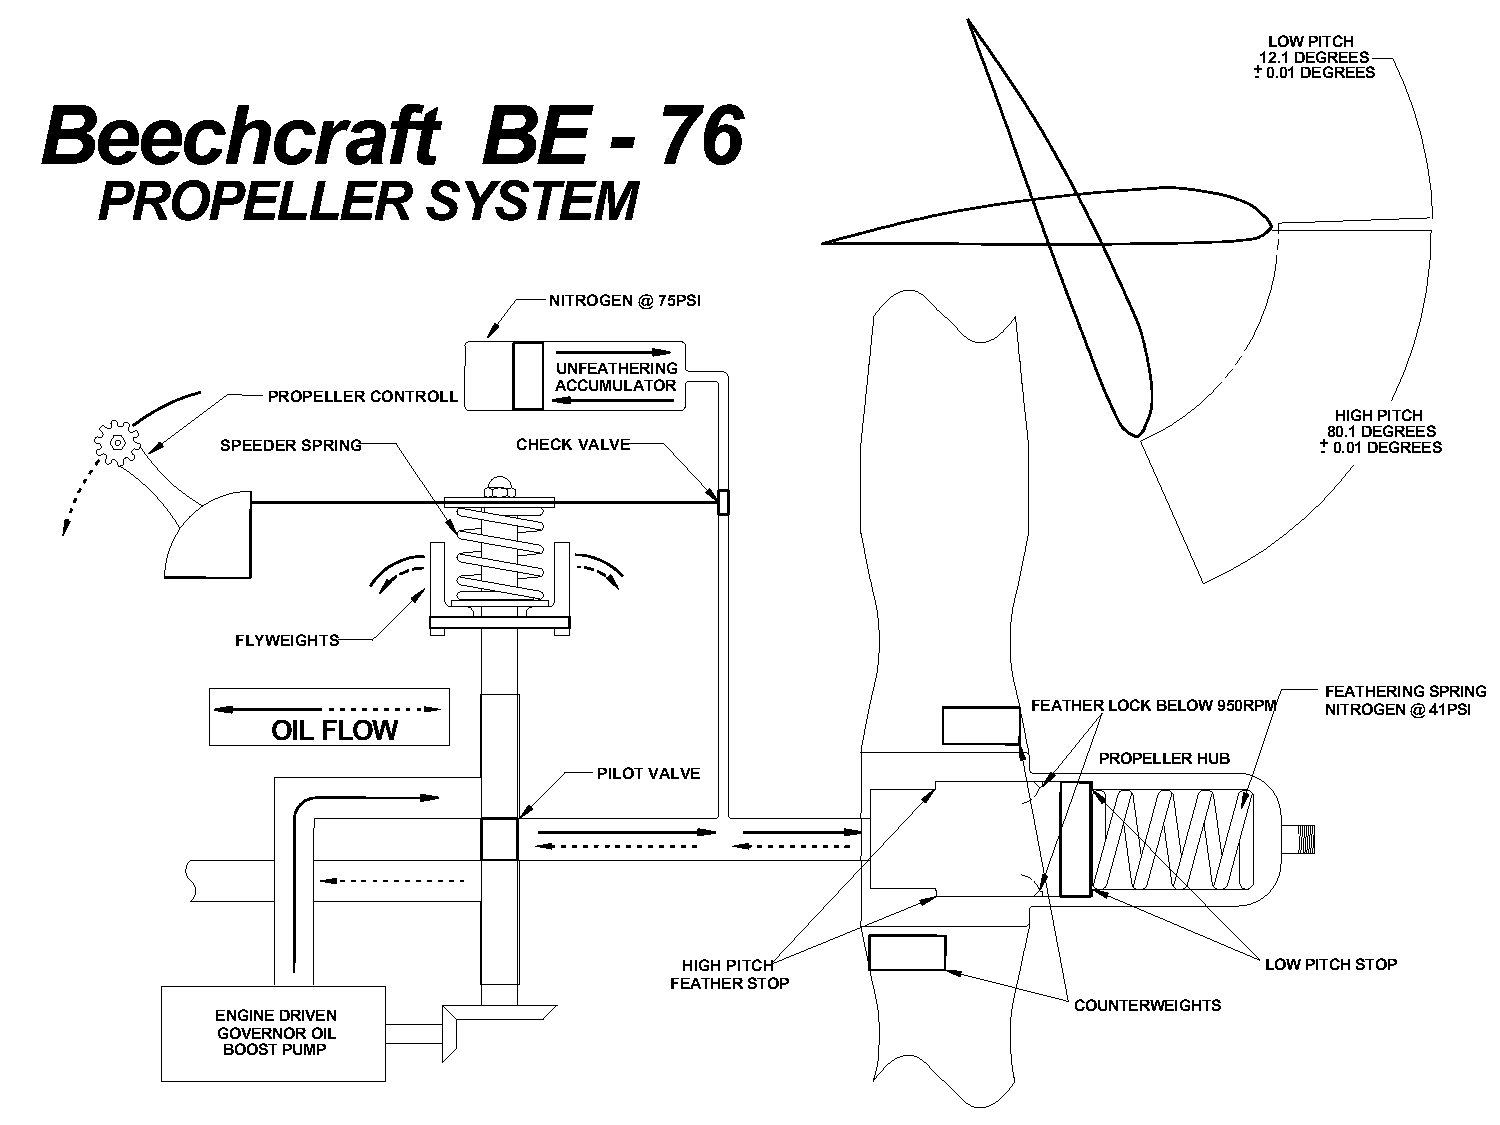
\includegraphics[width=1.0\linewidth]{be76-propeller}
\end{center}
\end{figure}

\newpage

\subsection{Landing Gear}

\begin{figure}[H]
\begin{center}
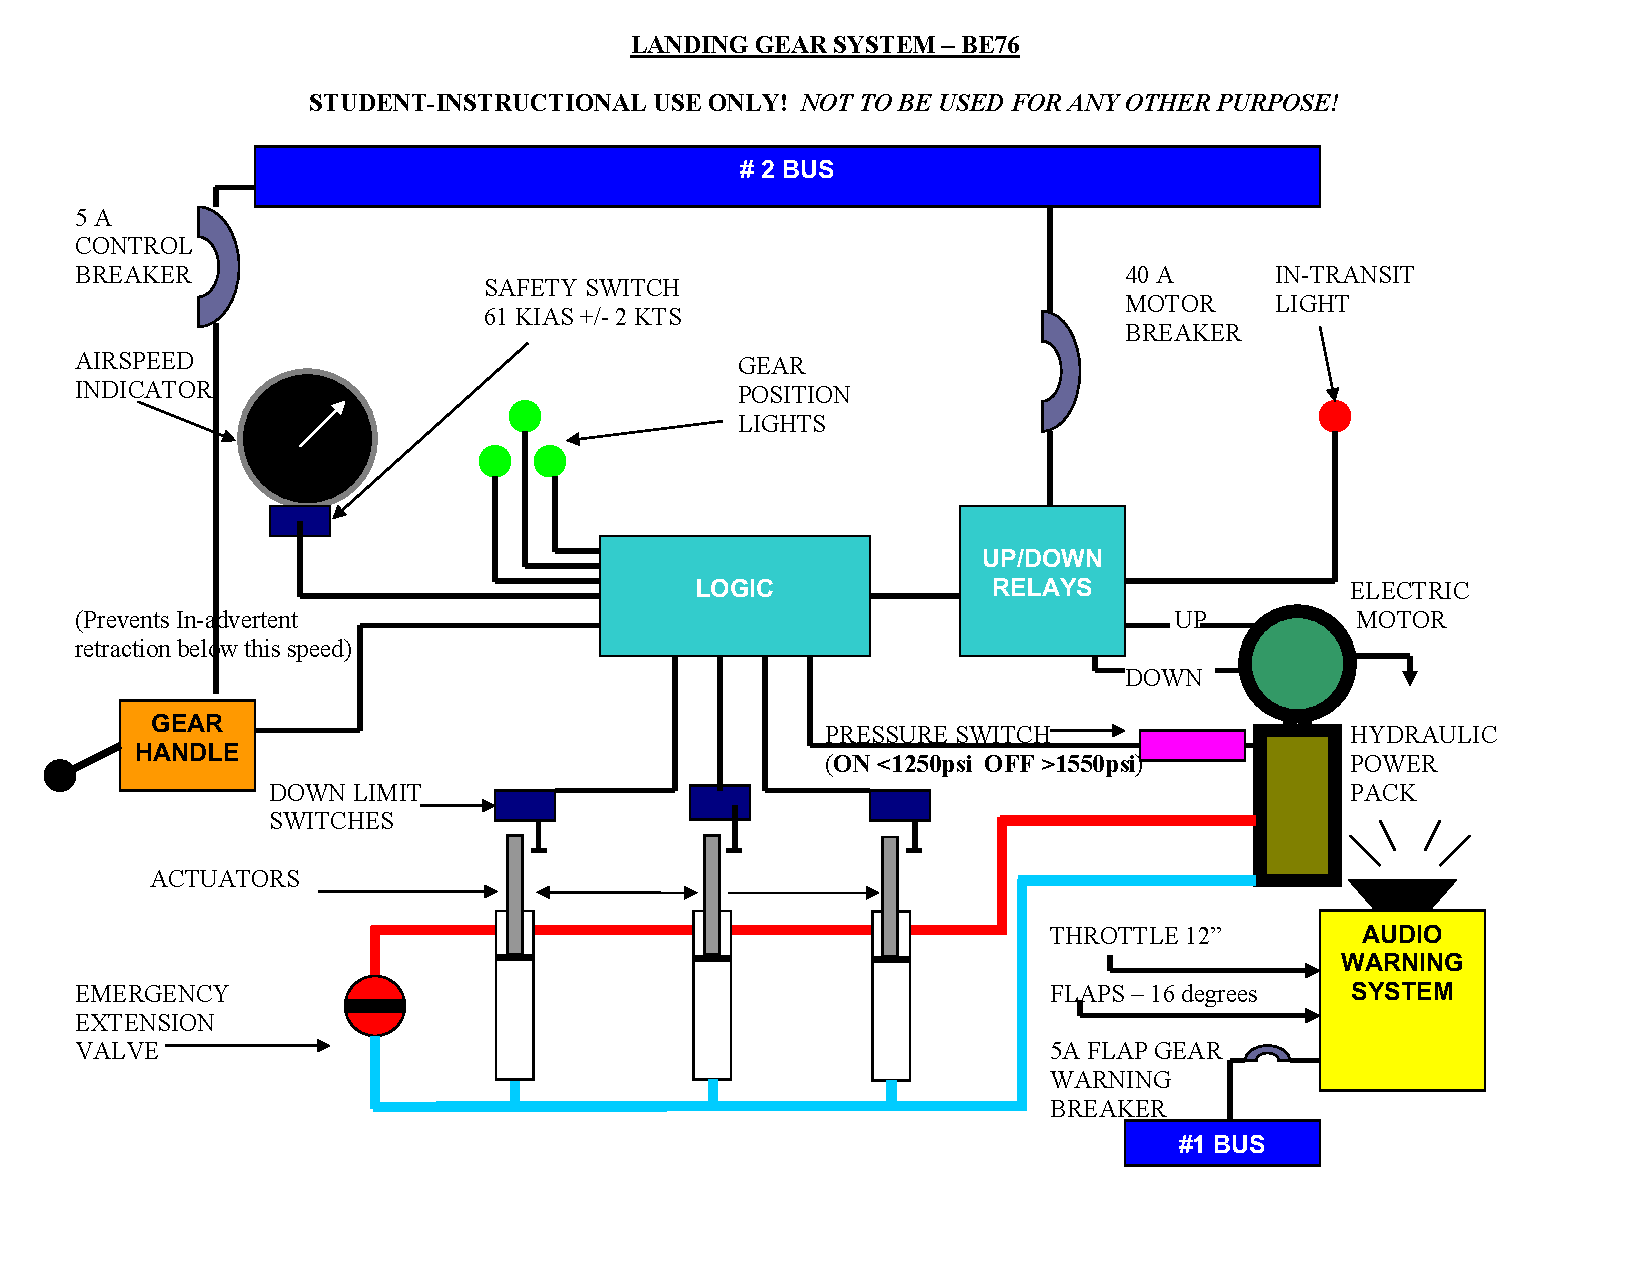
\includegraphics[trim={1cm 1cm 1cm 1cm},clip,width=1.0\linewidth]{be76-landinggear}
\end{center}
\end{figure}

\newpage


\subsection{Pressure System}

\begin{figure}[H]
\begin{center}
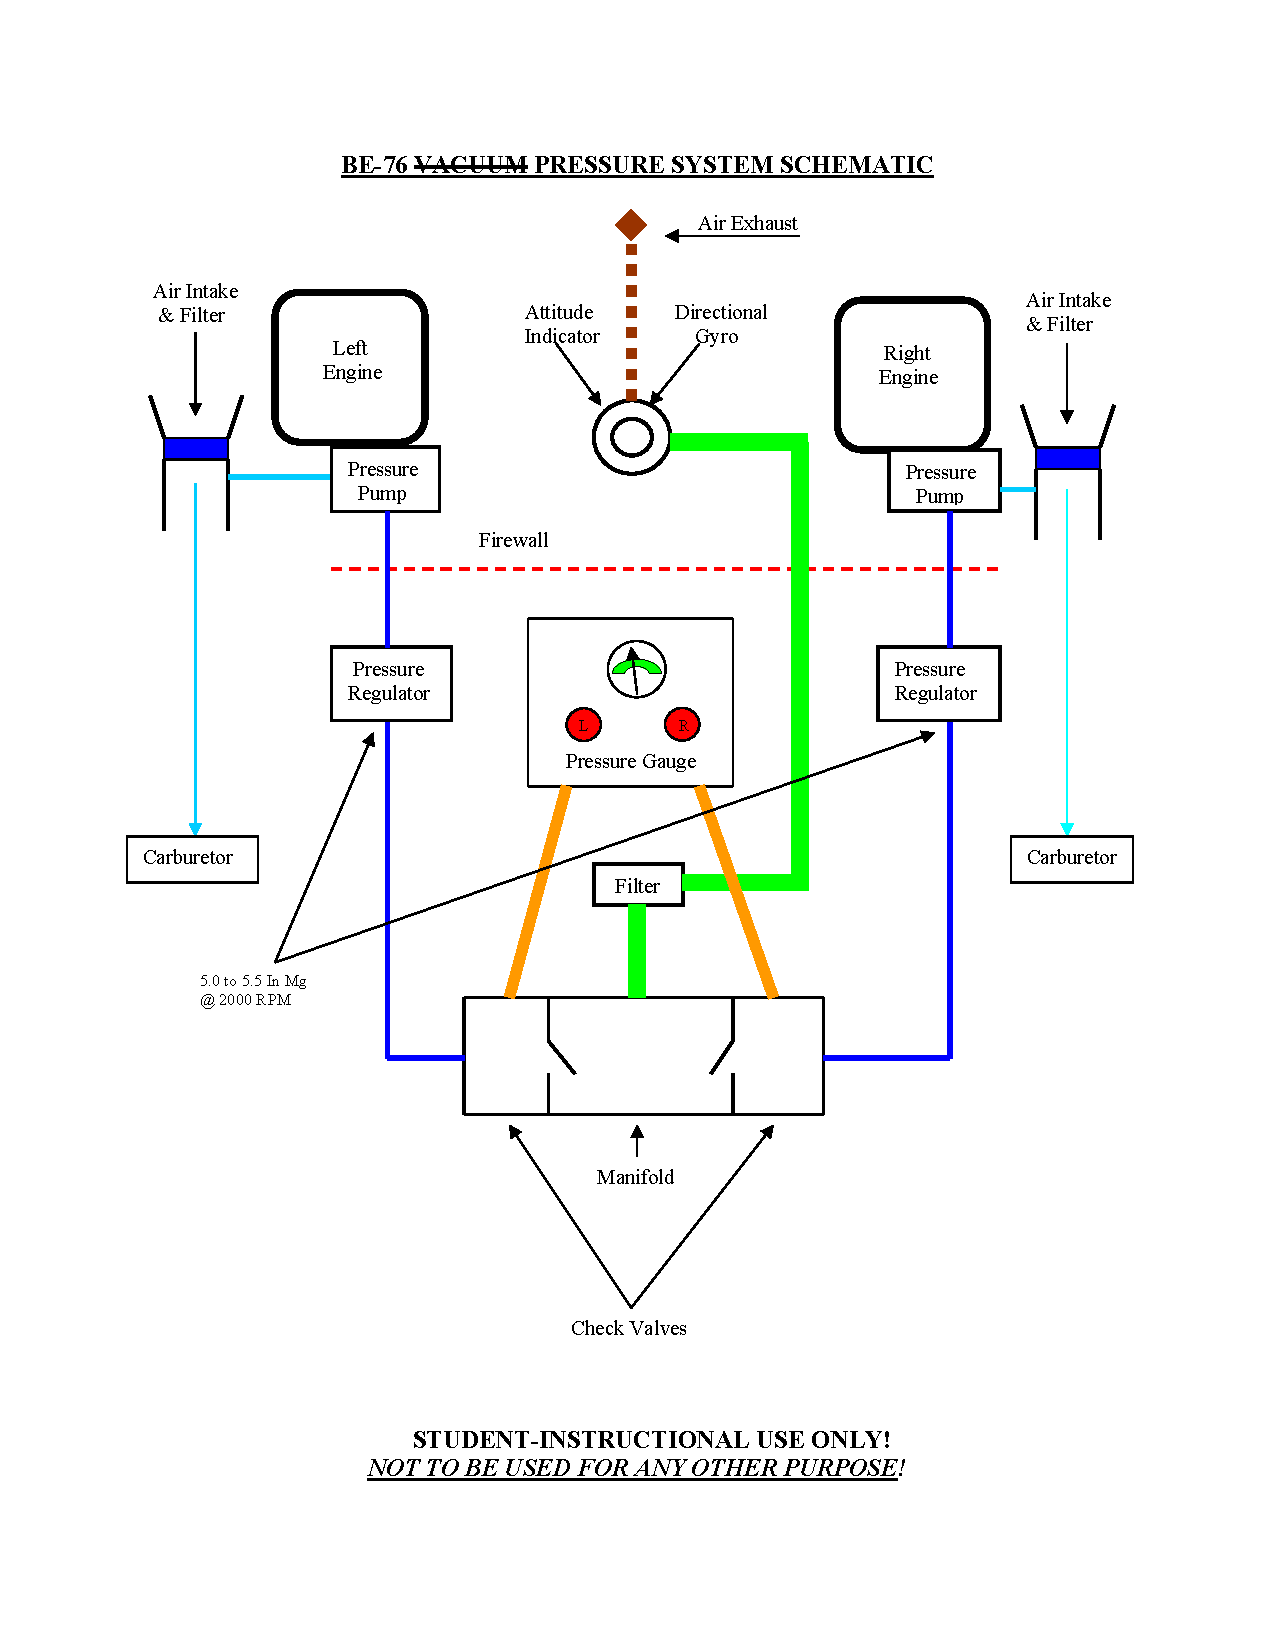
\includegraphics[trim={2cm 2cm 2cm 2cm},clip,width=0.9\linewidth]{be76-pressure}
\end{center}
\end{figure}


\subsection{Fuel System}

\begin{figure}[H]
\begin{center}
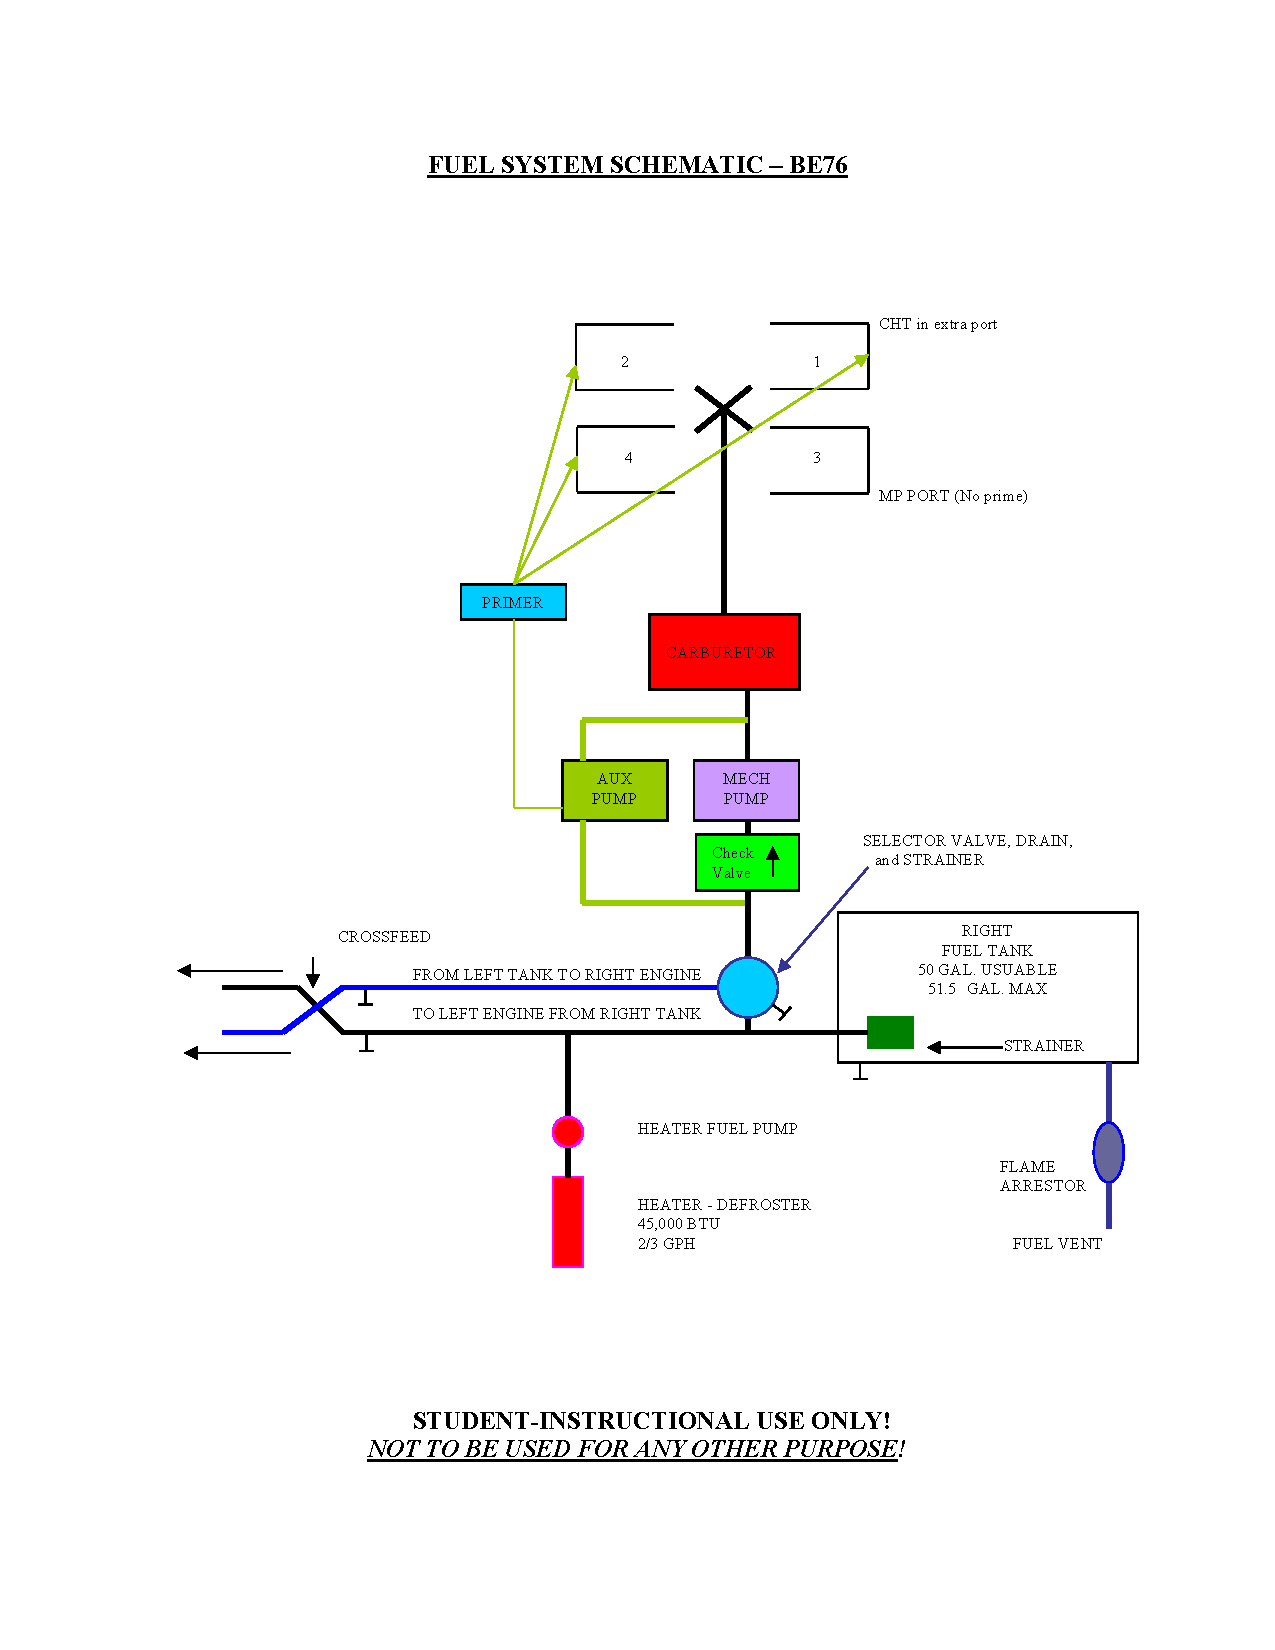
\includegraphics[trim={2cm 2cm 2cm 2cm},clip,width=0.9\linewidth]{be76-fuel}
\end{center}
\end{figure}


\subsection{Electrical System}

\begin{figure}[H]
\begin{center}
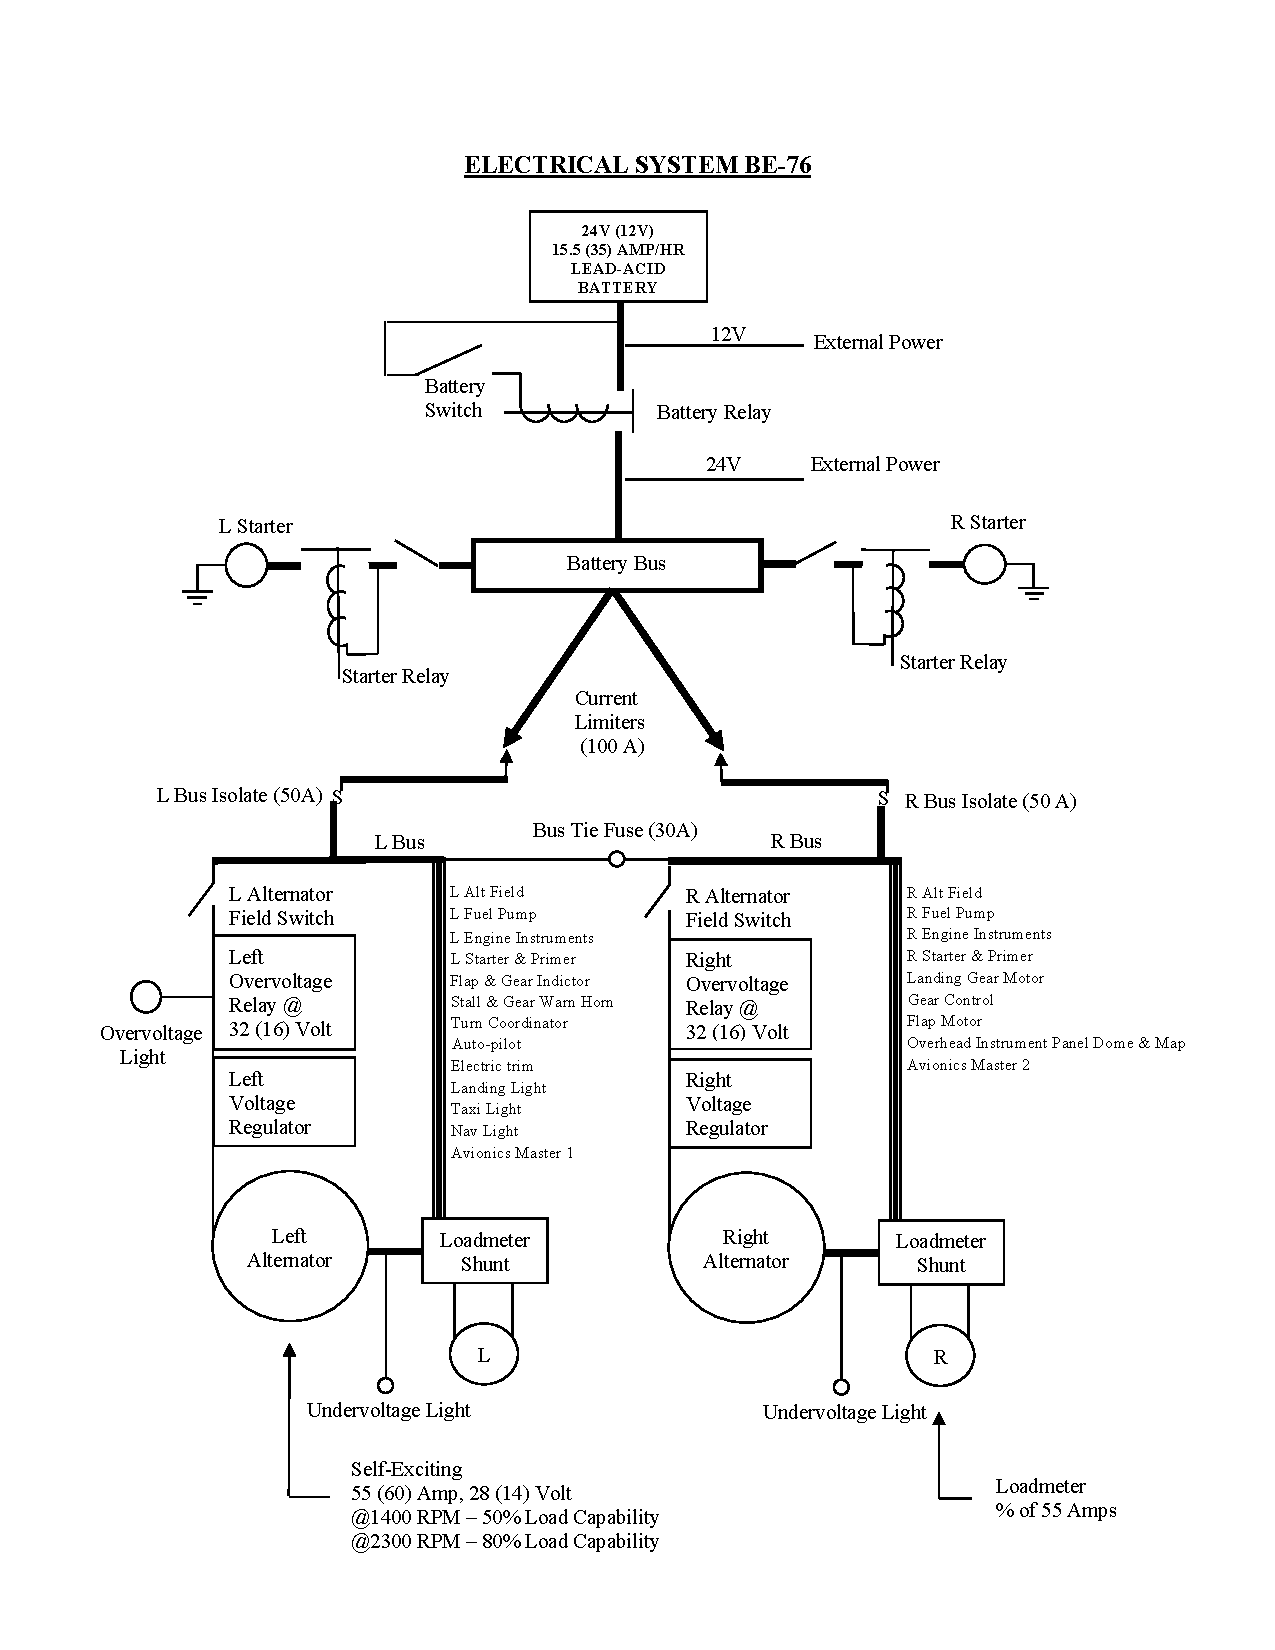
\includegraphics[trim={2cm 2cm 2cm 2cm},clip,width=0.9\linewidth]{be76-electrical}
\end{center}
\end{figure}

